\chapter{State-Management Ansätze}

Bei den populären SM Lösungen folgen Redux und NgRx dem Flux-Pattern\cite{historyOfRedux}\cite{ngrxGettingStarted}, wobei Zustand und Pinia einen anderen, Framework-nahen Ansatz verfolgen.

\section{Redux}

Im Folgenden wird die Funktionsweise und die Eigenschaften von Redux näher beschrieben. Diese gelten ebenfalls für NgRx.

Redux definiert sich durch folgenden frei Eigenschaften:
\begin{enumerate}
  \item Unveränderlichkeit (Immutability): Änderung am State sind ausschließlich über die APIs von Redux möglich.
  \item Zentralisierung des Zustandes: Der gesamte Applikationszustand lebt in einem zentral JavaScript Objekt.
  \item Nachvollzierbarkeit (Traceability): Während der gesamten Lebensdauer der Applikation sind Änderungen am Zustand auf deren Ursprung verfolgbar.
\end{enumerate}

Um dies zu erreichen, werden zwei verschienede APIs zur Verfügung gestellt. Diese sind \textit{actions} und \textit{reducer}. Außerdem können optionale \textit{selectors} benutzt werden um aus bestimmten Teilen des Zustandes zu lesen.

\subsection{Actions}

Eine Action (Aktion) beschreibt eine Änderung oder Interaktion in der und mit der Applikation. 

\begin{figure}[h!]
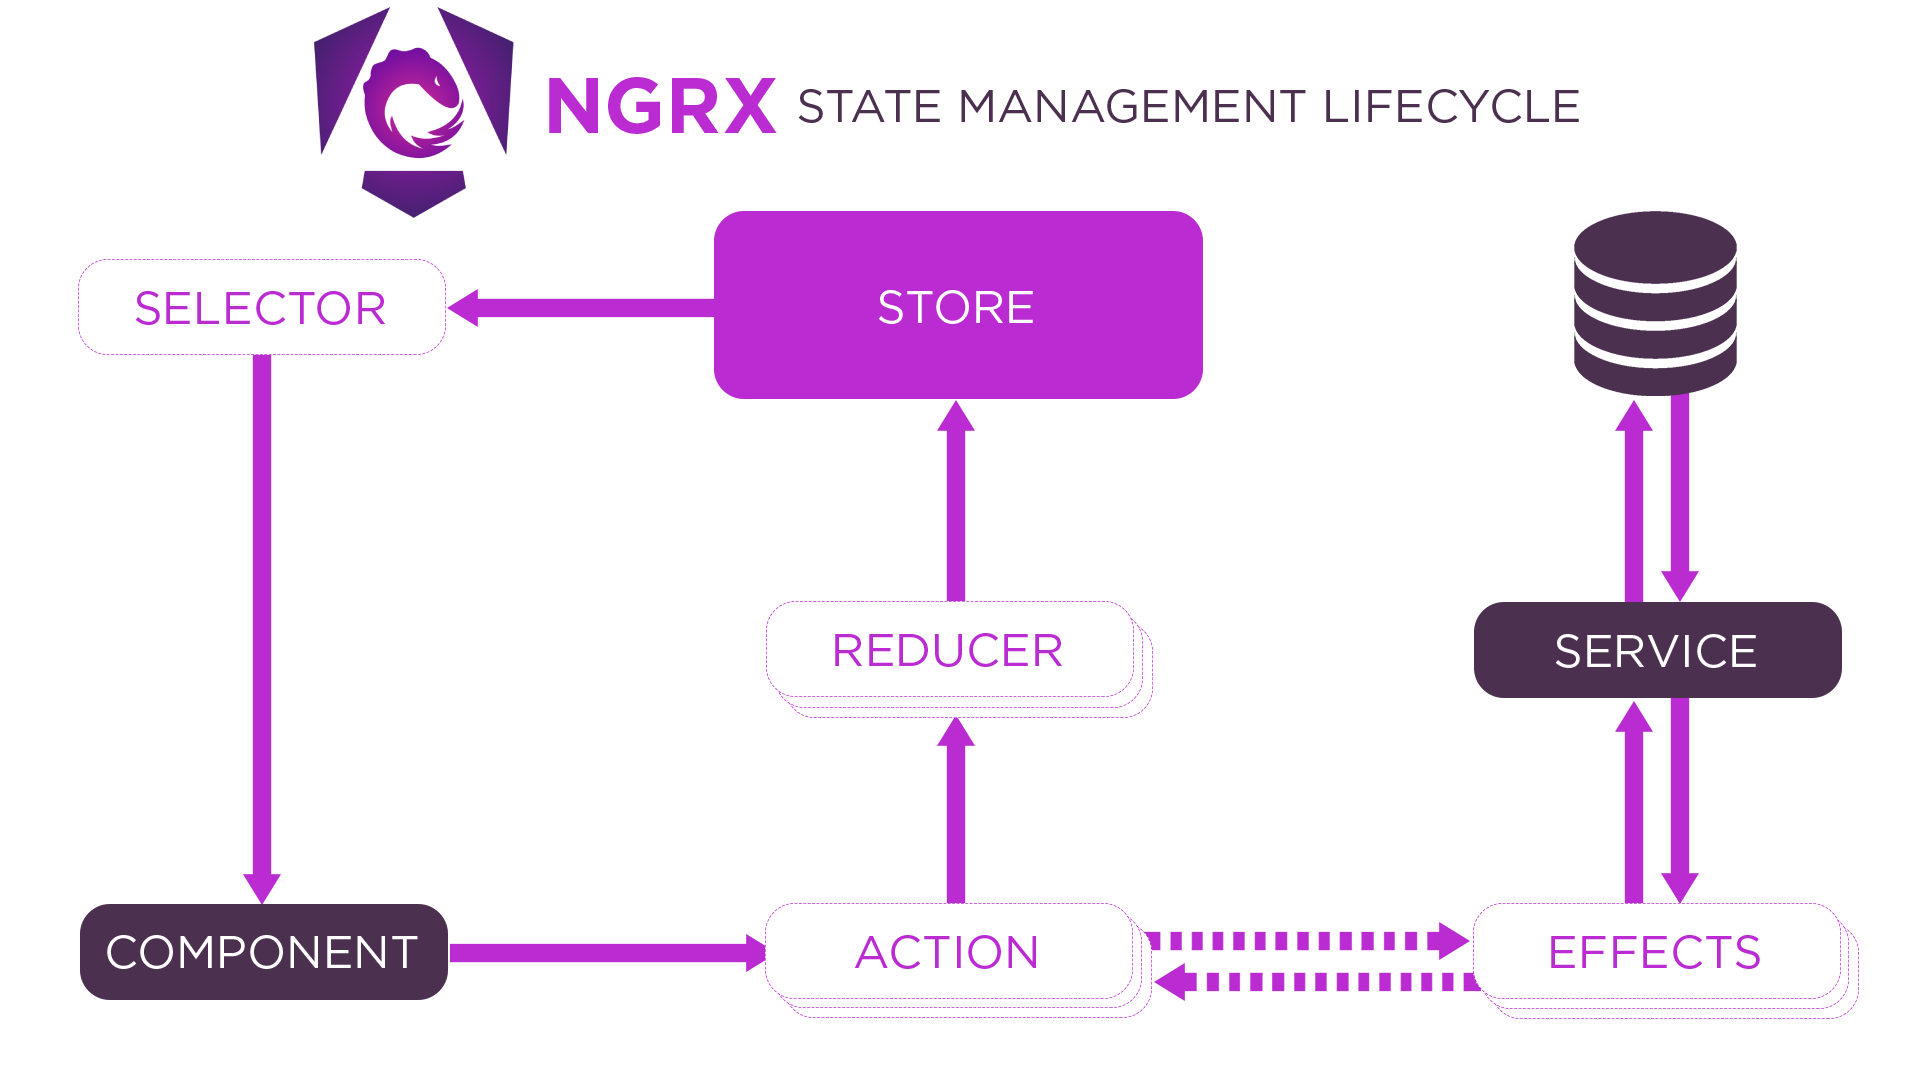
\includegraphics[width=1\textwidth]{state-management-lifecycle.png}
\caption{NgRx Datenfluss}
\end{figure}